%\documentclass[a4paper]{article}
\usepackage[utf8]{inputenc}
\usepackage[spanish, es-tabla, es-noshorthands]{babel}
\usepackage[table,xcdraw]{xcolor}
\usepackage[a4paper, footnotesep=1.25cm, headheight=1.25cm, top=2.54cm, left=2.54cm, bottom=2.54cm, right=2.54cm]{geometry}
%\geometry{showframe}

%\usepackage{wrapfig}			%Wrap figure in text
\usepackage[export]{adjustbox}	%Move images
\usepackage{changepage}			%Move tables

\usepackage{tikz}
\usepackage{amsmath}
\usepackage{amsfonts}
\usepackage{amssymb}
\usepackage{float}
\usepackage{graphicx}
\usepackage{caption}
\usepackage{subcaption}
\usepackage{multicol}
\usepackage{multirow}
\usepackage{wrapfig}
\setlength{\doublerulesep}{\arrayrulewidth}
\usepackage{booktabs}
\usepackage[numbib, nottoc, notlot, notlof]{tocbibind}

\usepackage{hyperref}
\hypersetup{
    colorlinks=true,
    linkcolor=blue,
    filecolor=magenta,      
    urlcolor=blue,
    citecolor=blue,    
}

%Change Font Size

% #1 = size, #2 = text
\newcommand{\setparagraphsize}[2]{{\fontsize{#1}{6}\selectfont#2 \par}}		%Cambia el size de todo el parrafo
\newcommand{\setlinesize}[2]{{\fontsize{#1}{6}\selectfont#2}}				%Cambia el font de una oración

\newcommand{\note}[1]{
	\begin{center}
		\huge{ \textcolor{red}{#1} }
	\end{center}
}

%FONTS (IMPORTANTE): Compilar en XeLaTex o LuaLaTeX
\usepackage{anyfontsize}	%Font size
\usepackage{fontspec}		%Font type

\usepackage{etoolbox}
\usepackage{todonotes}

\newcommand{\observacion}[2]{  \ifnumequal{1}{#1}{ { \todo[inline,backgroundcolor=red!25,bordercolor=red!100]{\textbf{Observación: #2}} } }{  }  }

\setcounter{topnumber}{2}
\setcounter{bottomnumber}{2}
\setcounter{totalnumber}{4}
\renewcommand{\topfraction}{0.85}
\renewcommand{\bottomfraction}{0.85}
\renewcommand{\textfraction}{0.15}
\renewcommand{\floatpagefraction}{0.8}
\renewcommand{\textfraction}{0.1}
\setlength{\floatsep}{5pt plus 2pt minus 2pt}
\setlength{\textfloatsep}{5pt plus 2pt minus 2pt}
\setlength{\intextsep}{5pt plus 2pt minus 2pt}

\newcommand{\quotes}[1]{``#1''}
\usepackage{array}
\newcolumntype{C}[1]{>{\centering\let\newline\\\arraybackslash\hspace{0pt}}m{#1}}
\usepackage[american]{circuitikz}
\usetikzlibrary{calc}
\usepackage{fancyhdr}
\usepackage{units} 

\graphicspath{{../Control de posición no lineal/}{../Control de fuerza no lineal/}{../Control híbrido no lineal/}{../Referencias/}{../Deducción de modelo/}{../Conclusiones/}}

\pagestyle{fancy}
\fancyhf{}
\lhead{22.99 - Automación Industrial}
\rhead{Lambertucci, Londero B., Maselli, Mechoulam}
\rfoot{Página \thepage}

%Items con bullets y no cuadrados
\renewcommand{\labelitemi}{\textbullet }


%\begin{document}

\subsection{Caracterización del problema}
A continuación se presenta el desarrollo de un control de fuerzas no lineal. Para ello un aspecto fundamental el modelo de las fuerzas del sistema que interaccionan con el actuador.

En este caso, la fuerza consiste en la pared que trabaja como obstáculo. La fuerza de reacción entre el EE y la pared es aquella definida por:
\begin{equation}
f_r = k_e \cdot d \ \hat{n}
\label{eq:fuerza_pared}
\end{equation}

La Ecuación (\ref{eq:fuerza_pared}) es una fuerza proporcional a la distancia y normal a la superficie de la pared. Esta es nula mientras el EE no se encuentre en contacto con la pared y no nula en caso de estarlo.

\subsection{Esquema de control propuesto}
El esquema de control propuesto es nuevamente una linealización por realimentación de la siguiente manera:

\begin{figure}[H]
	\centering
	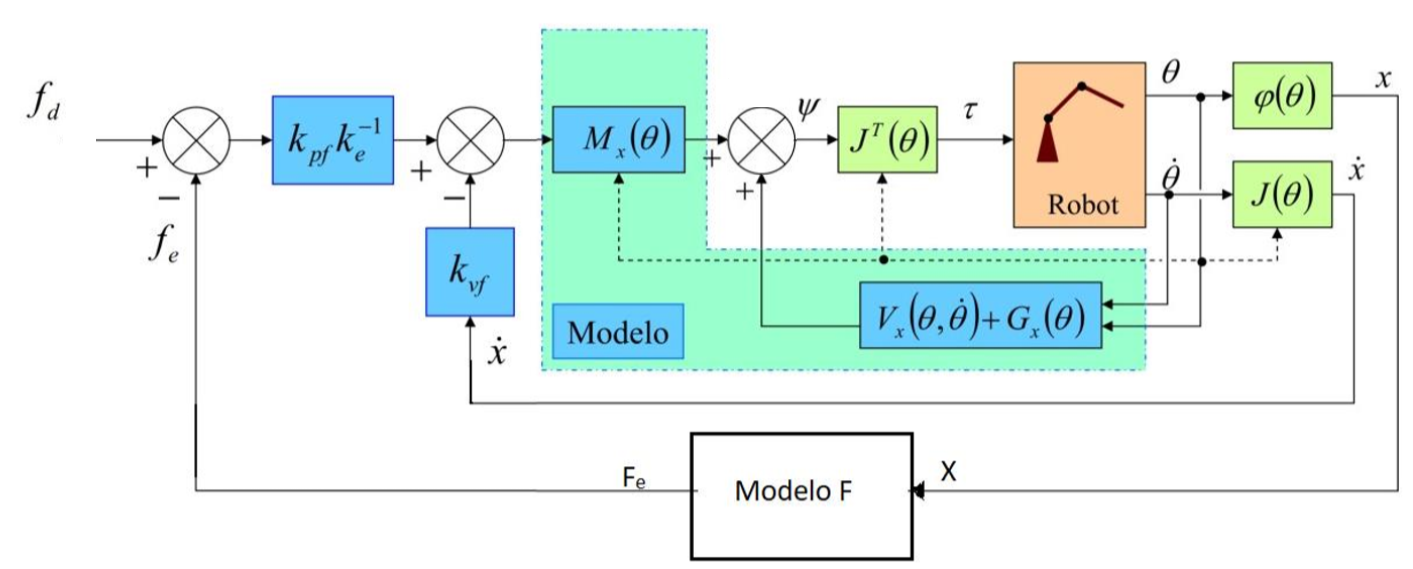
\includegraphics[width=0.8\linewidth]{ImagenesControl de fuerza no lineal/controlf}
	\caption{Topología del control de fuerza no lineal.}	
	\label{fig:control_f_modelo}
\end{figure}

\observacion{\verObs}{HABLAR DE VALORES DE GANANCIAS}

Nuevamente y de manera análoga lo presentado en las Secciones (\ref{sec:posic}) y (\ref{sec:fuerza}), se utilizó el método de Ziegler-Nichols. De esta forma, los valores obtenidos fueron:
\begin{itemize}
	\item Kv = [139 0;0 139].
	\item Kp = [420 0; 0 420].
\end{itemize}

\subsection{Resultados}
Nuevamente se realizó el simulink del sistema, obteniendo así los gráficos que se presentan a continuación.

Algo característico que tiene este control de fuerzas es que, debido a que no hay información provista como referencia de posición, el manipulador se mueve hasta encontrarse cerca de la pared. Luego realiza una breve oscilación sobre el obstáculo hasta llegar a un estado permanente en el cual el manipulador está aplicando la fuerza comandada por la referencia.

\begin{figure}[H]
	\centering
	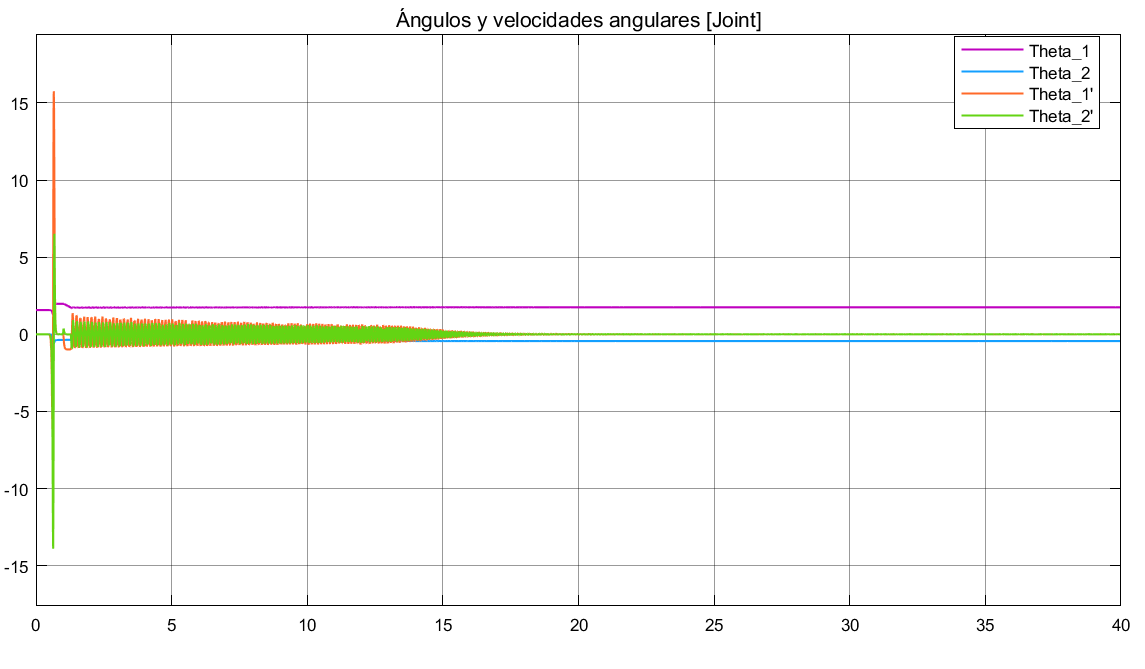
\includegraphics[width=0.8\linewidth]{ImagenesControl de fuerza no lineal/2_3_a}
	\caption{\'Angulos en función del tiempo en espacio joint.}	
	\label{fig:athetas_f}
\end{figure}

Se observa en la Figura (\ref{fig:apos_f}) la leve oscilación del EE al llegar a la pared.

\begin{figure}[H]
	\centering
	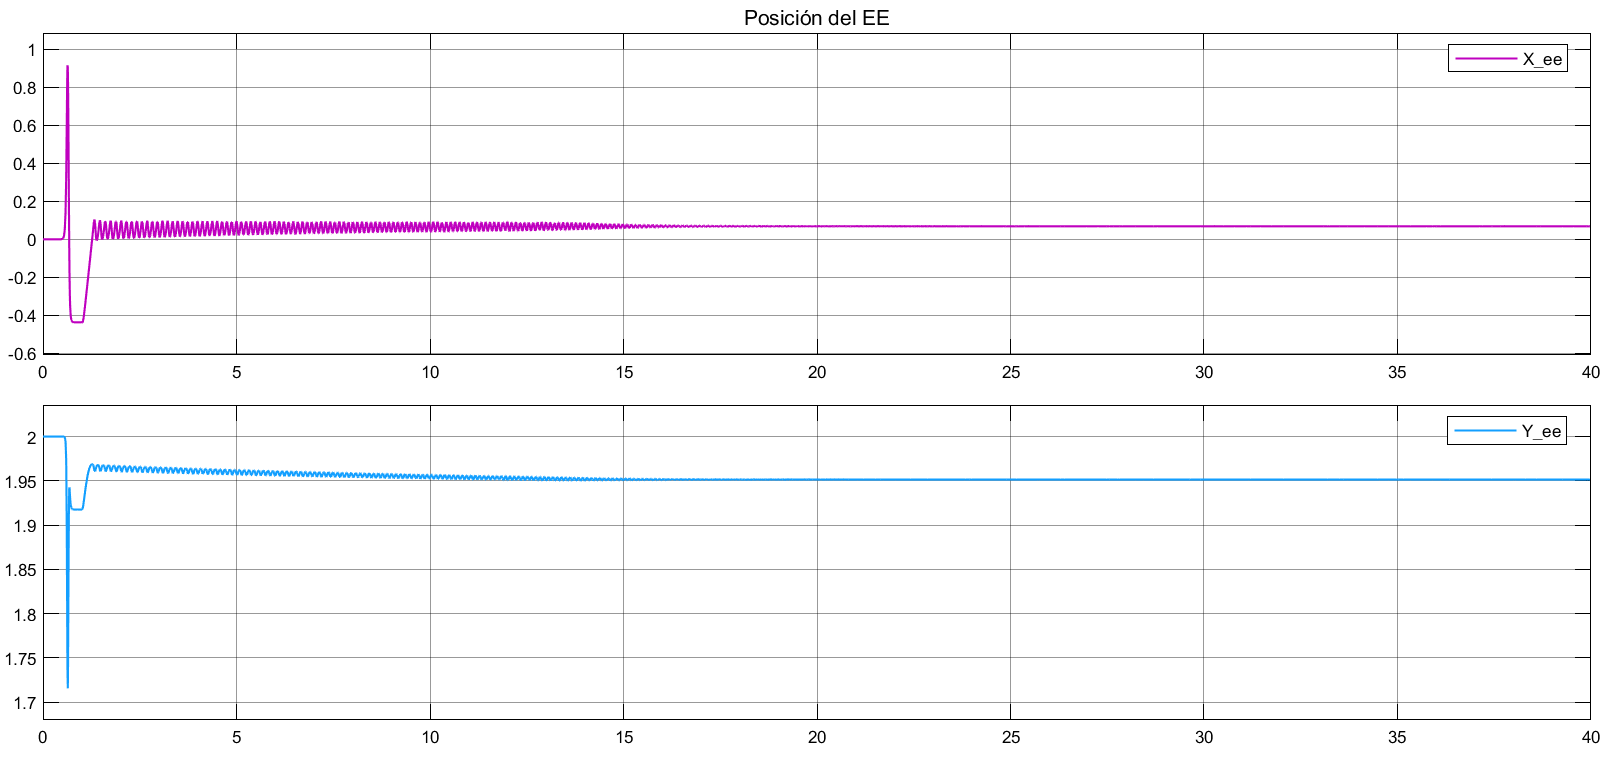
\includegraphics[width=0.8\linewidth]{ImagenesControl de fuerza no lineal/2_3_b}
	\caption{Posición  del EE.}	
	\label{fig:apos_f}
\end{figure}

\begin{figure}[H]
	\centering
	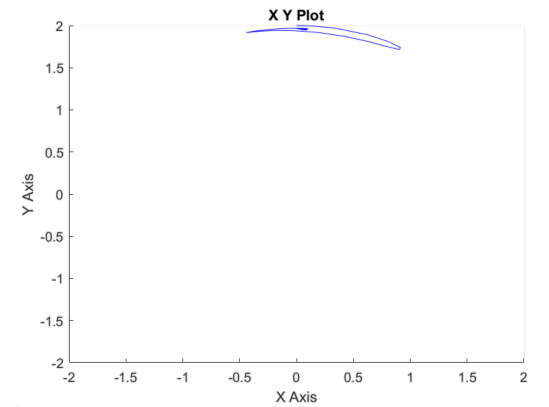
\includegraphics[width=0.5\linewidth]{ImagenesControl de fuerza no lineal/2_3_c}
	\caption{Gráfico XY.}	
	\label{fig:axy_f}
\end{figure}

Cabe mencionar en la Figura (\ref{fig:axy_f}) la función es nula en varios puntos. Esto se debe a que el manipulador no está en contacto con la pared por lo que la misma no aplica una fuerza.

Además se observa como una vez alcanzada la pared y dada una referencia, el EE oscila levemente en torno a la referencia hasta establecerse.

\begin{figure}[H]
	\centering
	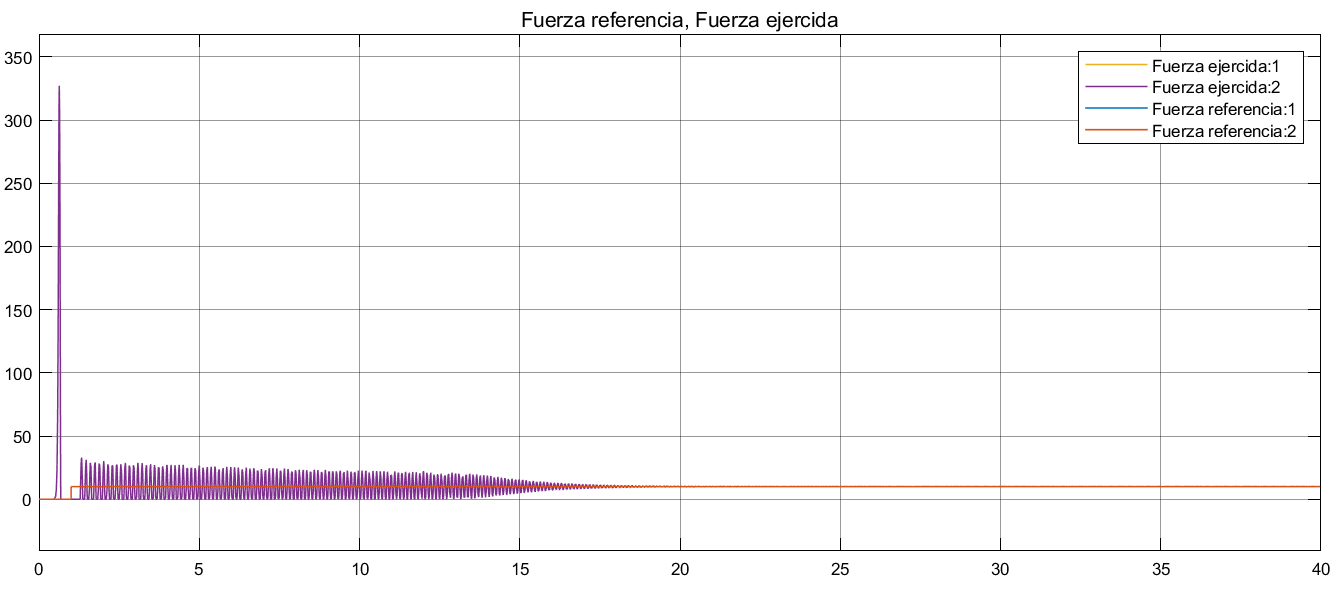
\includegraphics[width=0.8\linewidth]{ImagenesControl de fuerza no lineal/2_3_e}
	\caption{Fuerzas de referencia y ejercida.}	
	\label{fig:af_f}
\end{figure}

También se le incluyó un disturbio a la planta tanto en posición como en velocidad. Se puede ver en la Figura (\ref{fig:athetasd_f}) como el momento en el que se le aplica el disturbio a la planta las variables de estado se estabilizan nuevamente.
\begin{figure}[H]
	\centering
	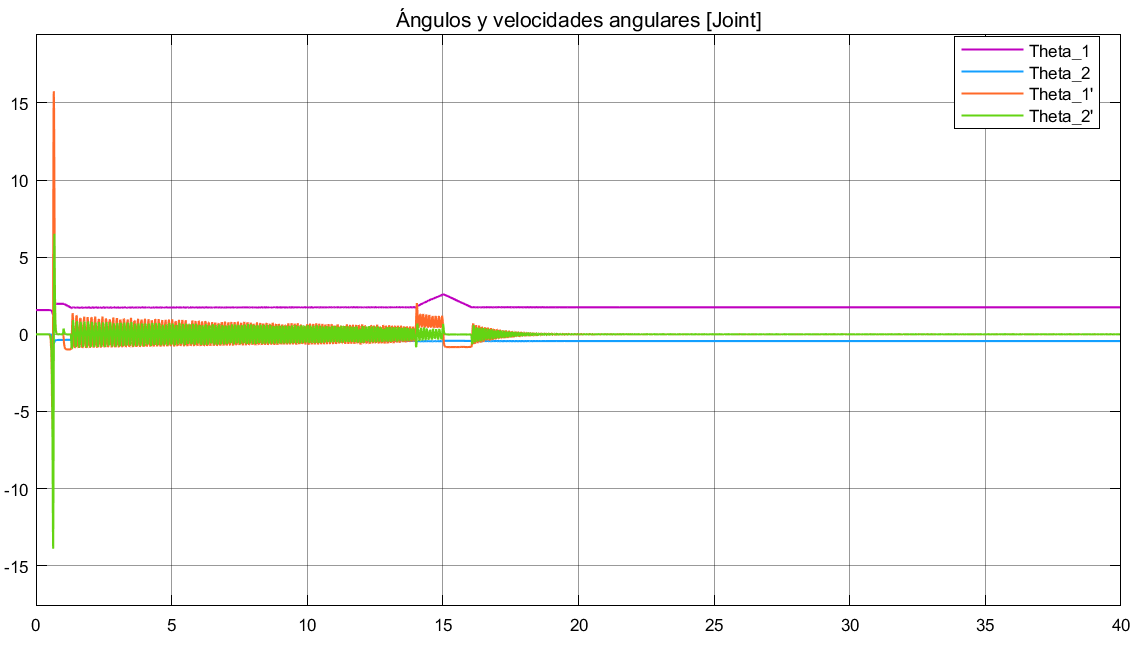
\includegraphics[width=0.8\linewidth]{ImagenesControl de fuerza no lineal/2_3_f_a}
	\caption{Ángulos en función del tiempo en espacio joint.}	
	\label{fig:athetasd_f}
\end{figure}

Luego se muestra el movimiento del EE.
\begin{figure}[H]
	\centering
	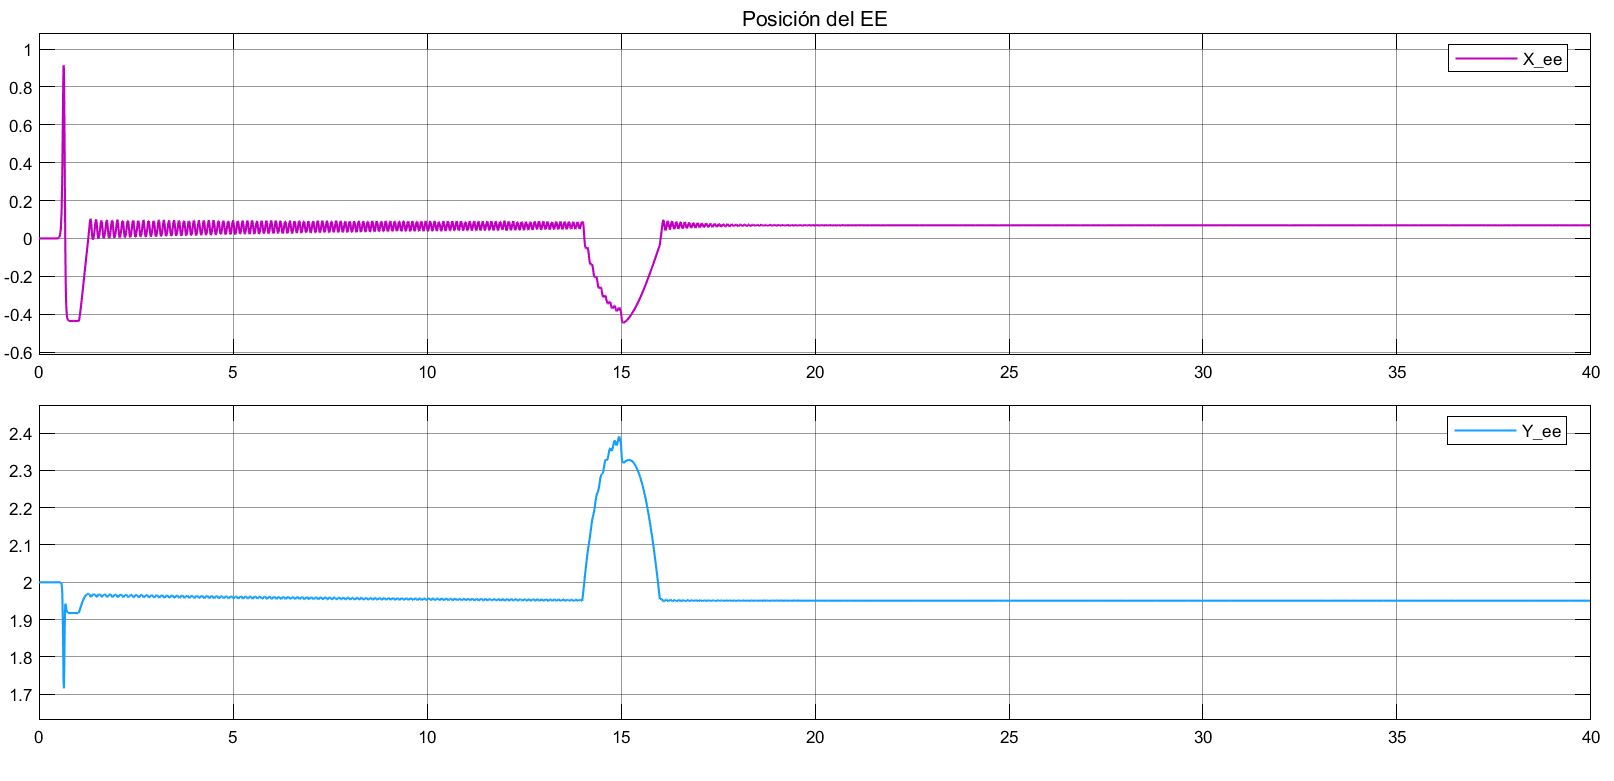
\includegraphics[width=0.8\linewidth]{ImagenesControl de fuerza no lineal/2_3_f_b}
	\caption{Posición del EE.}	
	\label{fig:aposd_f}
\end{figure}

\begin{figure}[H]
	\centering
	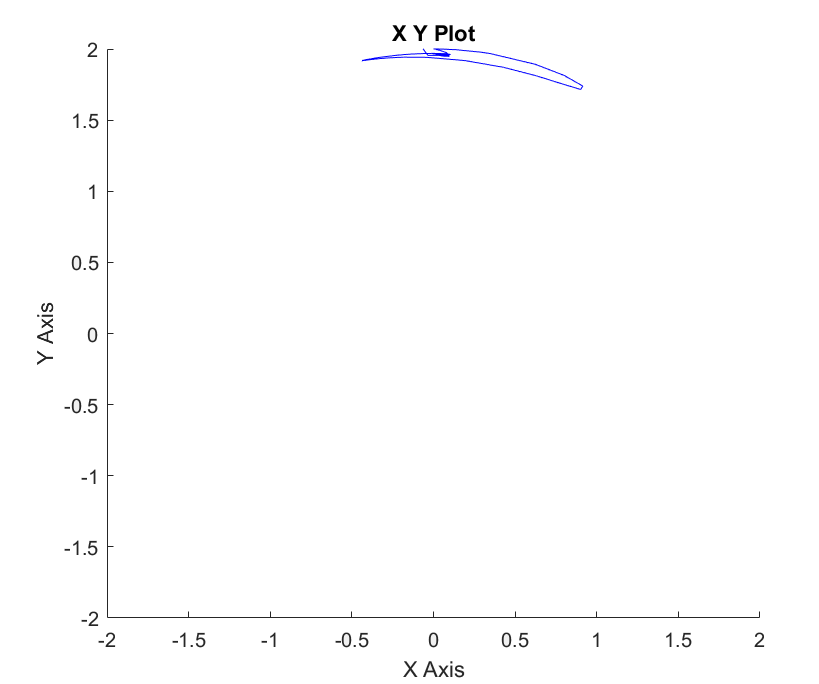
\includegraphics[width=0.5\linewidth]{ImagenesControl de fuerza no lineal/2_3_f_c}
	\caption{Gráfico XY.}	
	\label{fig:bxyd_f}
\end{figure}

Finalmente se observa un gráfico similar al de fuerzas anterior, con la diferencia de que se hace nulo el valor de la fuerza aplicada en el segundo 15. 

En dicho instante es el EE se despega completamente de la pared para luego volver a la misma. Es así que se establece en el régimen permanente nuevamente.

\begin{figure}[H]
	\centering
	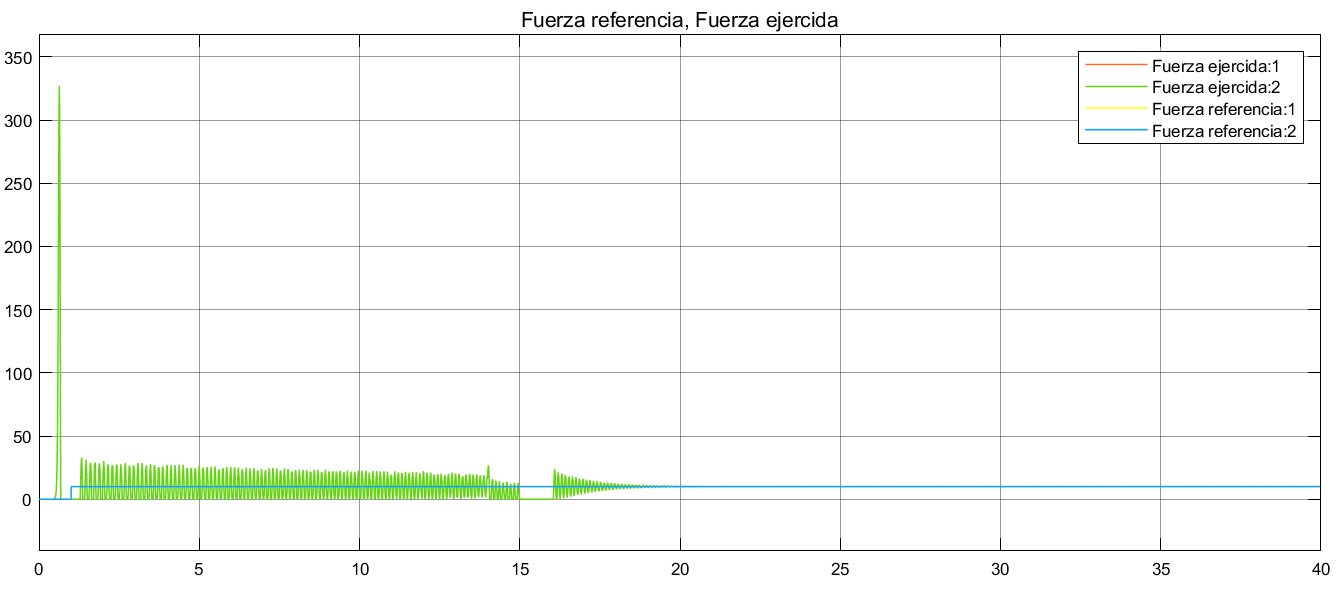
\includegraphics[width=0.8\linewidth]{ImagenesControl de fuerza no lineal/2_3_f_e}
	\caption{Fuerza deseada y real.}	
	\label{fig:bfd_f}
\end{figure}
%\end{document}
